\section{Komplexe Funktion, Abbildungen}
	\begin{minipage}[t]{0.5\textwidth}
		\subsection{Definition}
			\hfill\\
			\scalebox{0.5}{\begin{tikzpicture}
	\node[black!70!green] at (0.5, 5.7) {$z_1$};
	\node[black!70!green] at (0.5, 5) {$z_2$};
	\draw[->, black!70!green, very thick] (0.7, 5.7) -- (1, 5.4);
	\draw[->, black!70!green, very thick] (0.7, 5) -- (1, 5.3);
	\node[black!70!green] at (2.3, 5.35) {$z = z_1 + \mathrm{j} z_2$};
	\draw[->, black!70!green, very thick] (3.5, 5.35) -- (7, 5.35);
	
	\node[blue] at (16, 5.7) {$w_1$};
	\node[blue] at (16, 5) {$w_2$};
	\draw[->, blue, very thick] (15.3, 5.4) -- (15.6, 5.7);
	\draw[->, blue, very thick] (15.3, 5.3) -- (15.6, 5);
	\node[blue] at (14, 5.35) {$w = w_1 + \mathrm{j} w_2$};
	\draw[->, blue, very thick] (9.5, 5.35) -- (12.5, 5.35);
	
	\node[minimum size=2cm, draw] at (8.3, 5.35) {\scalebox{3}{$\textcolor{red}{f}$}};
	
	\draw[->, very thick, red] (22:8cm) arc[radius=1, start angle=140, end angle=40] node[above, red] at (8.3, 3.3) {$f$};
	\node[above, red] at (8.3, 3.8) {$z \rightarrowtail w = f(z)$};
	
	\node[above, font=\large\bfseries] at (1, 5.8) {$\underline{\text{z-Ebene:}}$};
	\begin{tikzpicture}
	\begin{axis}[
		axis lines=middle,
		axis equal,
		xmin=-2,
		xmax=2,
		ymin=-2,
		ymax=2,
		xlabel=$z_1$,
		ylabel=$z_2$,
		xticklabels={,,},
		yticklabels={,,}
	]
		\addplot[draw=none] coordinates {(1, 1)};
		\addplot[mark=*, black!70!green] coordinates {(-0.5, 0.5)} node[below, black!70!green] {$z$} node[above, black!70!green] {Orginalpunkt};
		\node at (axis cs:1.5, 1) {\scalebox{2.5}{\rom{1}}};
		\node at (axis cs:-1.5, 1) {\scalebox{2.5}{\rom{2}}};
		\node at (axis cs:-1.5, -1) {\scalebox{2.5}{\rom{3}}};
		\node at (axis cs:1.5, -1) {\scalebox{2.5}{\rom{4}}};
	\end{axis}
\end{tikzpicture}\hspace{2.7cm}%
	
	\node[above, font=\large\bfseries] at (1.2, 5.8) {$\underline{\text{w-Ebene:}}$};
	\begin{tikzpicture}
	\begin{axis}[
		axis lines=middle,
		axis equal,
		xmin=-2,
		xmax=2,
		ymin=-2,
		ymax=2,
		xlabel=$w_1$,
		ylabel=$w_2$,
		xticklabels={,,},
		yticklabels={,,}
	]
		\addplot[draw=none] coordinates {(1,1)};
		\addplot[mark=*, blue] coordinates {(0.5, -0.5)} node[below, blue] {$w$} node[above, blue] {Bildpunkt};
		\node at (axis cs:1.5, 1) {\scalebox{2.5}{\rom{1}}};
		\node at (axis cs:-1.5, 1) {\scalebox{2.5}{\rom{2}}};
		\node at (axis cs:-1.5, -1) {\scalebox{2.5}{\rom{3}}};
		\node at (axis cs:1.5, -1) {\scalebox{2.5}{\rom{4}}};
	\end{axis}
\end{tikzpicture}
\end{tikzpicture}}
	\end{minipage}
	\begin{minipage}[t]{0.5\textwidth}
		\subsection{Winkeltreue}
			Komplexe Funktion $f\left( z \right)$ ist in allen Punkten winkeltreu, wo gibt: \fbox{$f^{\prime}\left( z \right) \neq 0$}\\[6pt]
			Sie bewirkt \textbf{lokal eine Drehstreckung:}\\[3pt]
			\begin{tabular}{ll}
				Streckungsfaktor: & \fbox{$\left|f^{\prime}(z)\right|$}\\[3pt]
				Drehwinkel: & \fbox{$\operatorname{\arg}\left( z \right)$}\\[3pt]
				Verschieben: & \fbox{$f^{\prime}\left( z \right)$}
			\end{tabular}
	\end{minipage}

\subsection{Parameter- und Koordinatengleichung}
	\begin{minipage}[]{0.2\textwidth}
		\scalebox{0.5}{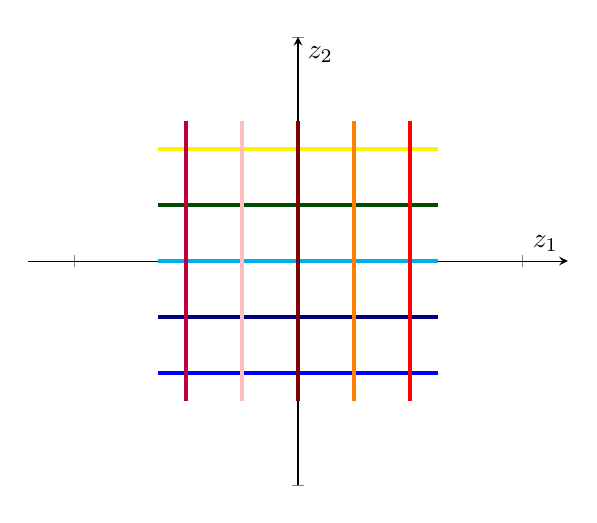
\begin{tikzpicture}
	\begin{axis}[
		axis lines=middle,
		axis equal,
		xmin=-4,
		xmax=4,
		ymin=-4,
		ymax=4,
		xlabel=$z_1$,
		ylabel=$z_2$,
		xticklabels={,,},
		yticklabels={,,}
	]
		\addplot[-, yellow, ultra thick] coordinates {(-2.5, 2) (2.5, 2)};
		\addplot[-, black!70!green, ultra thick] coordinates {(-2.5, 1) (2.5, 1)};
		\addplot[-, cyan, ultra thick] coordinates {(-2.5, 0) (2.5, 0)};
		\addplot[-, black!50!blue, ultra thick] coordinates {(-2.5, -1) (2.5, -1)};
		\addplot[-, blue, ultra thick] coordinates {(-2.5, -2) (2.5, -2)};
		
		\addplot[-, purple, ultra thick] coordinates {(-2, -2.5) (-2, 2.5)};
		\addplot[-, pink, ultra thick] coordinates {(-1, -2.5) (-1, 2.5)};
		\addplot[-, black!50!red, ultra thick] coordinates {(0, -2.5) (0, 2.5)};
		\addplot[-, orange, ultra thick] coordinates {(1, -2.5) (1, 2.5)};
		\addplot[-, red, ultra thick] coordinates {(2, -2.5) (2, 2.5)};
	\end{axis}
\end{tikzpicture}}
	\end{minipage}
	\begin{minipage}[]{0.8\textwidth}
		\begin{tabular}{llll}
			\textbf{waagrechte Gitternetzlinien durch Punkt $(0; c_2)$:} & & &
		\end{tabular}\\[3pt]
		\begin{tabular}{llll}
			\fbox{$z = \operatorname{z}\left( r \right) = r + \mathrm{j} c_2$} & $\xrightarrow[]{f\left( z \right)}$ & \fbox{$w = \operatorname{w}\left( r \right) = f\left( \operatorname{z}\left( r \right) \right) = f\left( r + \mathrm{j} c_2 \right)$} & mit $r \subset \mathbb{R}$\\[3pt]
		\end{tabular}\\[3pt]
		\begin{tabular}{llll}
			\textbf{senkrechte Gitternetzlinien durch Punkt $(c_1; 0)$:} & & &
		\end{tabular}
		\begin{tabular}{llll}
			\fbox{$z = \operatorname{z}\left( r \right) = c_1 + \mathrm{j} r$} & $\xrightarrow[]{f\left( z \right)}$ & \fbox{$w = \operatorname{w}\left( r \right) = f\left( \operatorname{z}\left( r \right) \right) = f\left( c_1 + \mathrm{j} r \right)$} & mit $r \subset \mathbb{R}$\\[3pt]
		\end{tabular}
		\begin{tabular}{llll}
			\textbf{Koordinatengleichung:} & 
			\fbox{$\left| \begin{array}{c}
				w_1 = \operatorname{Re}\left(\left[ f\left(\operatorname{z}\left(r \right)\right)\right]\right)\\[3pt]
				w_2 = \operatorname{Re}\left(\left[ f\left(\operatorname{z}\left(r \right)\right)\right]\right)
				\end{array} \right|$} &
			$\Rightarrow$ & 
			$\begin{array}{l}
				\text{Parameter $r$ eliminieren,}\\[3pt]
				\text{um Koordinatengleichung}\\[3pt]
				\text{zu erhalten.}
			\end{array}$
		\end{tabular}
	\end{minipage}

\subsection{Lineare Funktion}
	\begin{minipage}[]{0.5\textwidth}
		\scalebox{0.5}{\begin{tikzpicture}	
	\draw[->, very thick, red] (22:8cm) arc[radius=1, start angle=140, end angle=40] node[above, red] at (8.3, 3.3) {$z \rightarrowtail w = f(z)$} node at (8.3, 2.3) {$f(z) = a \cdot z + b$};
	
	\begin{tikzpicture}
	\begin{axis}[
		axis lines=middle,
		axis equal,
		xmin=-4,
		xmax=4,
		ymin=-4,
		ymax=4,
		xlabel=$z_1$,
		ylabel=$z_2$,
		xticklabels={,,},
		yticklabels={,,}
	]
		\addplot[-, yellow, ultra thick] coordinates {(-2.5, 2) (2.5, 2)};
		\addplot[-, black!70!green, ultra thick] coordinates {(-2.5, 1) (2.5, 1)};
		\addplot[-, cyan, ultra thick] coordinates {(-2.5, 0) (2.5, 0)};
		\addplot[-, black!50!blue, ultra thick] coordinates {(-2.5, -1) (2.5, -1)};
		\addplot[-, blue, ultra thick] coordinates {(-2.5, -2) (2.5, -2)};
		
		\addplot[-, purple, ultra thick] coordinates {(-2, -2.5) (-2, 2.5)};
		\addplot[-, pink, ultra thick] coordinates {(-1, -2.5) (-1, 2.5)};
		\addplot[-, black!50!red, ultra thick] coordinates {(0, -2.5) (0, 2.5)};
		\addplot[-, orange, ultra thick] coordinates {(1, -2.5) (1, 2.5)};
		\addplot[-, red, ultra thick] coordinates {(2, -2.5) (2, 2.5)};
	\end{axis}
\end{tikzpicture}\hspace{2.7cm}%
	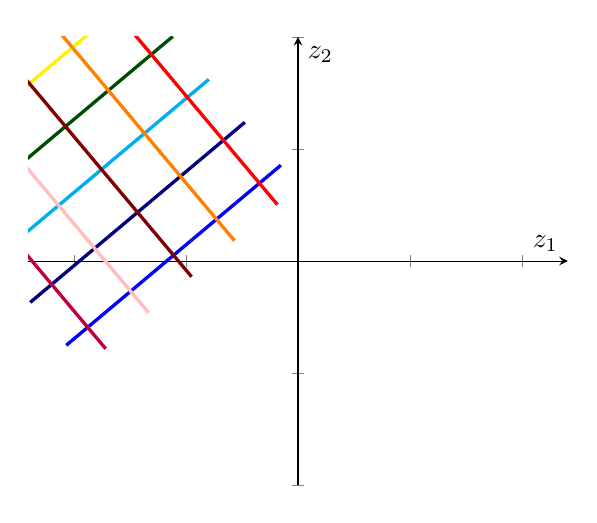
\begin{tikzpicture}
	\begin{axis}[
		axis lines=middle,
		axis equal,
		xmin=-4,
		xmax=4,
		ymin=-4,
		ymax=4,
		xlabel=$z_1$,
		ylabel=$z_2$,
		xticklabels={,,},
		yticklabels={,,}
	]
		\addplot[-, yellow, very thick, rotate=40] coordinates {(-2.5, 2) (2.5, 2)};
		\addplot[-, black!70!green, very thick, rotate=40] coordinates {(-2.5, 1) (2.5, 1)};
		\addplot[-, cyan, very thick, rotate=40] coordinates {(-2.5, 0) (2.5, 0)};
		\addplot[-, black!50!blue, very thick, rotate=40] coordinates {(-2.5, -1) (2.5, -1)};
		\addplot[-, blue, very thick, rotate=40] coordinates {(-2.5, -2) (2.5, -2)};
		
		\addplot[-, purple, very thick, rotate=40] coordinates {(-2, -2.5) (-2, 2.5)};
		\addplot[-, pink, very thick, rotate=40] coordinates {(-1, -2.5) (-1, 2.5)};
		\addplot[-, black!50!red, very thick, rotate=40] coordinates {(0, -2.5) (0, 2.5)};
		\addplot[-, orange, very thick, rotate=40] coordinates {(1, -2.5) (1, 2.5)};
		\addplot[-, red, very thick, rotate=40] coordinates {(2, -2.5) (2, 2.5)};
	\end{axis}
\end{tikzpicture}
\end{tikzpicture}}
	\end{minipage}
	\begin{minipage}[]{0.5\textwidth}
		Die lineare Funktion $w = f\left( z \right) = a z + b$ bewirkt:\\[3pt]
		\renewcommand{\arraystretch}{1.7}
		\begin{tabular}{|lll|}
			\hline
			Drehstreckung mit: & Streckungsfaktor & $\left|a\right|$\\
	 & Drehwinkel & $\operatorname{arg}\left( a \right)$\\
	 & Zentrum & $\dfrac{b}{1-a}$\\[6pt]
			\hline
			Drehstreckung mit: & Streckungsfaktor & $\left|a\right|$\\
			& Drehwinkel & $\operatorname{arg}\left( a \right)$\\
			\textbf{und} Translation um: & Ortsvektor & $b$\\
			\hline
		\end{tabular}
	\renewcommand{\arraystretch}{1}
	\end{minipage}\\[3pt]
	\begin{minipage}[t]{0.7\textwidth}
		\textbf{Parametergleichung:}\\[3pt]
		\begin{tabular}{lcl}
			Waagrechte & $\xrightarrow[]{f\left( z \right)}$ & $w = w(r) = \underbrace{\left( \mathrm{j} a c_2 + b \right)}_{Startvektor} + \hspace{25pt} r \cdot \hspace{-28pt} \underbrace{a}_{Richtungsvektor}$\\[3pt]
			Senkrechte & $\xrightarrow[]{f\left( z \right)}$ & $w = w(r) = \underbrace{\left( a c_1 + b \right)}_{Startvektor} + \hspace{25pt} r \cdot \hspace{-25pt} \underbrace{\mathrm{j}a}_{Richtungsvektor}$\\[3pt]
		\end{tabular}
	\end{minipage}
	\begin{minipage}[t]{0.3\textwidth}
		\textbf{Parametergleichung:}\\[3pt]
		$f^{\prime}\left( z \right) = a$\\[3pt]
		\begin{tabular}{ll}
			$\Rightarrow$ & für $a \neq 0$ ist $f\left( z \right) = a z + b$\\[3pt]
	 & \textbf{überall winkeltreu!}
		\end{tabular}
	\end{minipage}

\section{Potenzfunktion und Wurzelfunktion}
	\subsection{Quadratfunktion $z^2$ und Wurzelfunktion $\sqrt{z}$}
		Beim Quadrieren wird das \textbf{Argument verdoppelt} $\Rightarrow$ halbe $z$-Ebene füllt bereits die ganze $w$-Ebene aus.\\[3pt]
		\begin{minipage}[t]{0.5\textwidth}
			\scalebox{0.5}{\begin{tikzpicture}	
	\draw[->, very thick, red] (22:8cm) arc[radius=1, start angle=140, end angle=40] node[above, red] at (8.3, 3.3) {$w = z^2$};
	
	\begin{tikzpicture}
	\begin{axis}[
		axis lines=middle,
		axis equal,
		xmin=-5,
		xmax=5,
		ymin=-5,
		ymax=5,
		xlabel=$z_1$,
		ylabel=$z_2$,
	]
		\addplot[-, yellow, very thick] coordinates {(0, 4) (5, 4)};
		\addplot[-, white!40!orange, very thick] coordinates {(0, 3) (5, 3)};
		\addplot[-, white!20!orange, very thick] coordinates {(0, 2) (5, 2)};
		\addplot[-, white!5!orange, very thick] coordinates {(0, 1) (5, 1)};
		\addplot[-, orange, very thick] coordinates {(0, 0) (5, 0)};
		\addplot[-, white!40!red, very thick] coordinates {(0, -1) (5, -1)};
		\addplot[-, white!20!red, very thick] coordinates {(0, -2) (5, -2)};
		\addplot[-, white!5!red, very thick] coordinates {(0, -3) (5, -3)};
		\addplot[-, red, very thick] coordinates {(0, -4) (5, -4)};
		
		\addplot[-, purple, very thick] coordinates {(0, -5) (0, 5)};
		\addplot[-, white!50!purple, very thick] coordinates {(1, -5) (1, 5)};
		\addplot[-, blue, very thick] coordinates {(2, -5) (2, 5)};
		\addplot[-, white!50!blue, very thick] coordinates {(3, -5) (3, 5)};
		\addplot[-, cyan, very thick] coordinates {(4, -5) (4, 5)};
		
		\addplot[-{Triangle[width=18pt,length=8pt]}, line width=10pt, black!30!white] coordinates {(-2, 3) (-2, 1)};
		\addplot[-, line width=10pt, black!30!white] coordinates {(-0.5, 3) (-2.35, 3)};
		
		\addplot[-{Triangle[width=18pt,length=8pt]}, line width=10pt, black!30!white] coordinates {(-2, -3) (-2, -1)};
		\addplot[-, line width=10pt, black!30!white] coordinates {(-0.5, -3) (-2.35, -3)};
	\end{axis}
\end{tikzpicture}\hspace{2.7cm}%
	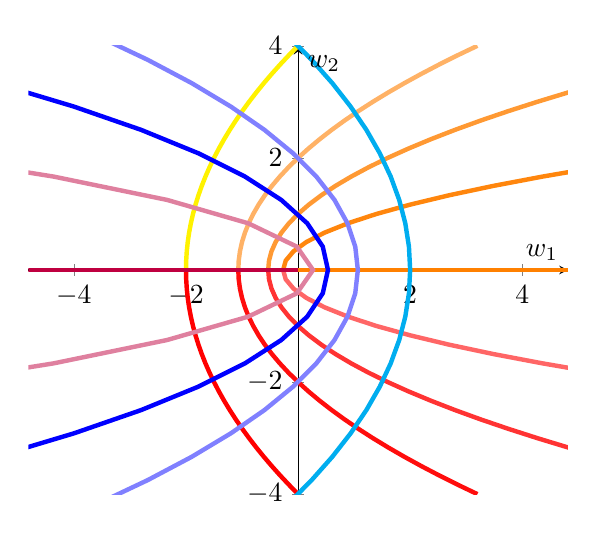
\begin{tikzpicture}
	\begin{axis}[
		axis lines=middle,
		axis equal,
		xmin=-4,
		xmax=4,
		ymin=-4,
		ymax=4,
		xlabel=$w_1$,
		ylabel=$w_2$,
	]
		
		\addplot[-, orange, ultra thick] coordinates {(0, 0) (5, 0)};
		
		\addplot[-, white!40!red, ultra thick, domain=-4:0] ({5/3*x^2 - 4/15},{x});
		\addplot[-, white!20!red, ultra thick, domain=-4:0] ({8/15*x^2 - 8/15},{x});
		\addplot[-, white!5!red, ultra thick, domain=-4:0] ({4/15*x^2 - 16/15},{x});
		\addplot[-, red, ultra thick, domain=-4:0] ({1/8*x^2 - 2},{x});
		
		\addplot[-, white!5!orange, ultra thick, domain=0:4] ({5/3*x^2 - 4/15},{x});
		\addplot[-, white!20!orange, ultra thick, domain=0:4] ({8/15*x^2 - 8/15},{x});
		\addplot[-, white!40!orange, ultra thick, domain=0:4] ({4/15*x^2 - 16/15},{x});
		\addplot[-, yellow, ultra thick, domain=0:4] ({1/8*x^2 - 2},{x});
		
		\addplot[-, purple, ultra thick] coordinates {(0, 0) (-5, 0)};
		
		\addplot[-, white!50!purple, ultra thick] ({-5/3*x^2 + 4/15},{x});
		\addplot[-, blue, ultra thick] ({-8/15*x^2 + 8/15},{x});
		\addplot[-, white!50!blue, ultra thick] ({-4/15*x^2 + 16/15},{x});
		\addplot[-, cyan, ultra thick] ({-1/8*x^2 + 2},{x});
	\end{axis}
\end{tikzpicture}
\end{tikzpicture}}
		\end{minipage}
		\begin{minipage}[t]{0.5\textwidth}
			\scalebox{0.5}{\begin{tikzpicture}	
	\draw[->, very thick, red] (22:8cm) arc[radius=1, start angle=140, end angle=40] node[above, red] at (8.3, 3.3) {$w = z^2$};
	
	\begin{tikzpicture}
	\begin{axis}[
		axis lines=middle,
		axis equal,
		xmin=-1.1,
		xmax=1.1,
		ymin=-1.1,
		ymax=1.1,
		xlabel=$z_1$,
		ylabel=$z_2$
	]	
		\addplot [domain=-90:90, samples=100, color=yellow] ({cos(x)}, {sin(x)});
		\addplot [domain=-90:90, samples=100, color=white!40!orange] ({4/5*cos(x)}, {4/5*sin(x)});
		\addplot [domain=-90:90, samples=100, color=white!20!orange] ({3/5*cos(x)}, {3/5*sin(x)});
		\addplot [domain=-90:90, samples=100, color=white!50!red] ({2/5*cos(x)}, {2/5*sin(x)});
		\addplot [domain=-90:90, samples=100, color=red] ({1/5*cos(x)}, {1/5*sin(x)});
		
		\addplot[-, blue, very thick] coordinates {(0, 1.1) (0, -1.1)};
		\addplot[-, white!40!blue, very thick] coordinates {(0, 0) ({1.1*cos(75)}, {1.1*sin(75)})};
		\addplot[-, white!60!blue, very thick] coordinates {(0, 0) ({1.1*cos(60)}, {1.1*sin(60)})};
		\addplot[-, white!80!blue, very thick] coordinates {(0, 0) ({1.1*cos(45)}, {1.1*sin(45)})};
		\addplot[-, white!60!cyan, very thick] coordinates {(0, 0) ({1.1*cos(30)}, {1.1*sin(30)})};
		\addplot[-, white!80!cyan, very thick] coordinates {(0, 0) ({1.1*cos(15)}, {1.1*sin(15)})};
		
		\addplot[-, purple, very thick] coordinates {(0, 0) (1.1, 0)};
		\addplot[-, cyan, very thick, dashed] coordinates {(0, 0) (1.1, 0)};
		
		\addplot[-, white!40!purple, very thick] coordinates {(0, 0) ({1.1*cos(-15)}, {1.1*sin(-15)})};
		\addplot[-, white!60!purple, very thick] coordinates {(0, 0) ({1.1*cos(-30)}, {1.1*sin(-30)})};
		\addplot[-, white!80!purple, very thick] coordinates {(0, 0) ({1.1*cos(-45)}, {1.1*sin(-45)})};
		\addplot[-, white!80!blue, very thick] coordinates {(0, 0) ({1.1*cos(-60)}, {1.1*sin(-60)})};
		\addplot[-, white!60!blue, very thick] coordinates {(0, 0) ({1.1*cos(-75)}, {1.1*sin(-75)})};
		
		\addplot[-{Triangle[width=18pt,length=8pt]}, line width=10pt, black!30!white] coordinates {(-0.5, 0.57) (-0.5, 0.15)};
		\addplot[-, line width=10pt, black!30!white] coordinates {(-0.1, 0.5) (-0.5, 0.5)};
		
		\addplot[-{Triangle[width=18pt,length=8pt]}, line width=10pt, black!30!white] coordinates {(-0.5, -0.57) (-0.5, -0.15)};
		\addplot[-, line width=10pt, black!30!white] coordinates {(-0.1, -0.5) (-0.5, -0.5)};
	\end{axis}
\end{tikzpicture}\hspace{2.7cm}%
	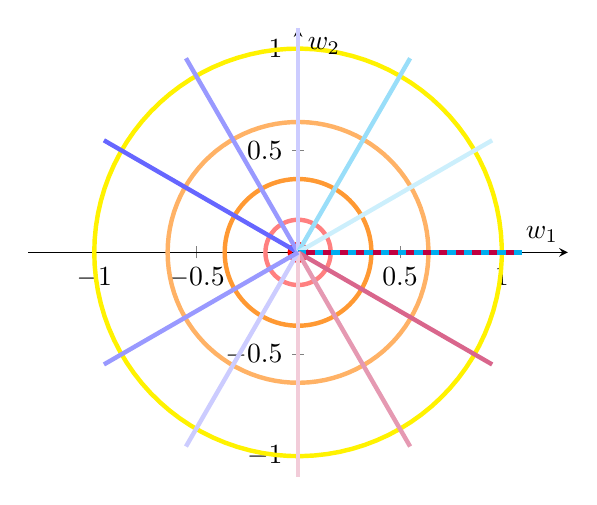
\begin{tikzpicture}
	\begin{axis}[
		axis lines=middle,
		axis equal,
		xmin=-1.1,
		xmax=1.1,
		ymin=-1.1,
		ymax=1.1,
		xlabel=$w_1$,
		ylabel=$w_2$
	]
		\addplot [domain=-180:180, samples=100, color=yellow, ultra thick] ({cos(x)}, {sin(x)});
		\addplot [domain=-180:180, samples=100, color=white!40!orange, ultra thick] ({(4/5)^2*cos(x)}, {(4/5)^2*sin(x)});
		\addplot [domain=-180:180, samples=100, color=white!20!orange, ultra thick] ({(3/5)^2*cos(x)}, {(3/5)^2*sin(x)});
		\addplot [domain=-180:180, samples=100, color=white!50!red, ultra thick] ({(2/5)^2*cos(x)}, {(2/5)^2*sin(x)});
		\addplot [domain=-180:180, samples=100, color=red, ultra thick] ({(1/5)^2*cos(x)}, {(1/5)^2*sin(x)});
		
		\addplot[-, blue, ultra thick] coordinates {(0, 1.1) (0, -1.1)};
		\addplot[-, white!40!blue, ultra thick] coordinates {(0, 0) ({1.1*cos(150)}, {1.1*sin(150)})};
		\addplot[-, white!60!blue, ultra thick] coordinates {(0, 0) ({1.1*cos(120)}, {1.1*sin(120)})};
		\addplot[-, white!80!blue, ultra thick] coordinates {(0, 0) ({1.1*cos(90)}, {1.1*sin(90)})};
		\addplot[-, white!60!cyan, ultra thick] coordinates {(0, 0) ({1.1*cos(60)}, {1.1*sin(60)})};
		\addplot[-, white!80!cyan, ultra thick] coordinates {(0, 0) ({1.1*cos(30)}, {1.1*sin(30)})};
		
		\addplot[-, purple, ultra thick] coordinates {(0, 0) (1.1, 0)};
		\addplot[-, cyan, ultra thick, dashed] coordinates {(0, 0) (1.1, 0)};
		
		\addplot[-, white!40!purple, ultra thick] coordinates {(0, 0) ({1.1*cos(-30)}, {1.1*sin(-30)})};
		\addplot[-, white!60!purple, ultra thick] coordinates {(0, 0) ({1.1*cos(-60)}, {1.1*sin(-60)})};
		\addplot[-, white!80!purple, ultra thick] coordinates {(0, 0) ({1.1*cos(-90)}, {1.1*sin(-90)})};
		\addplot[-, white!80!blue, ultra thick] coordinates {(0, 0) ({1.1*cos(-120)}, {1.1*sin(-120)})};
		\addplot[-, white!60!blue, ultra thick] coordinates {(0, 0) ({1.1*cos(-150)}, {1.1*sin(-150)})};
	\end{axis}
\end{tikzpicture}
\end{tikzpicture}}
		\end{minipage}
		\begin{minipage}[]{0.5\textwidth}
			\begin{framed}
				Die Quadratfunktion $w = f\left( z \right) = z^2$ bildet die\\[3pt]
				$z$-Ebene bijektiv \textbf{auf eine zweiblättrige\\[3pt] Riemann'sche Fläche ab}.
			\end{framed}
		\end{minipage}
		\begin{minipage}[]{0.5\textwidth}
			\scalebox{1.7}{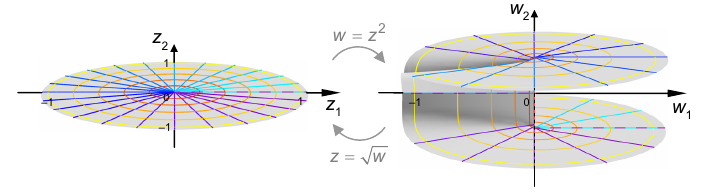
\includegraphics[width=0.5\textwidth]{pics/KomplexeZahlen/QuadratFunktion.png}}
		\end{minipage}\\[3pt]
		\begin{minipage}[]{0.15\textwidth}
			\textbf{Winkeltreue:}
		\end{minipage}
		\begin{minipage}[]{0.5\textwidth}
			\begin{framed}
				\begin{tabular}{lll}
					$f^{\prime}\left( z \right) = 2 z$ & $\Rightarrow$ & \textbf{winkeltreu} ausser bei $z = 0$\\[3pt]
					$f^{-1}\left( w \right) = \sqrt{w}$ & $\Rightarrow$ & \textbf{winkeltreu} ausser bei $w = 0$\\[3pt]
				\end{tabular}
			\end{framed}
		\end{minipage}
		\begin{minipage}[]{0.35\textwidth}
			\underline{\textbf{Winkeltreu $\rightarrow$ Vorgehen:}}
			\begin{enumerate}
				\item $\frac{d}{dz} (f(z))$
				\item $f^{\prime}\left( z \right) = 0$
				\item umformen $\Rightarrow$ Lösung: \underline{nicht} winkeltreu
			\end{enumerate}
		\end{minipage}\\[3pt]
	
	\subsection{Potenzfunktion $z^n$ und Wurzelfunktion $\sqrt[n]{z}$}
		\begin{minipage}[]{0.5\textwidth}
			\begin{framed}
				Die Potenzfunktion $w = f\left( z \right) = z^n$ bildet die\\[3pt]
				$z$-Ebene bijektiv \textbf{auf eine n-blättrige\\[3pt] Riemann'sche Fläche ab}.
			\end{framed}
		\end{minipage}
		\begin{minipage}[]{0.5\textwidth}
			\scalebox{1.7}{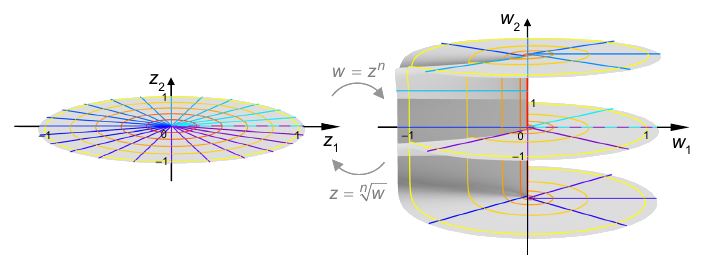
\includegraphics[width=0.5\textwidth]{pics/KomplexeZahlen/PotenzFunktion.png}}
		\end{minipage}\\[3pt]
	
\section{Kreisspiegelung}
	\begin{minipage}[]{0.5\textwidth}
		\begin{tabular}{lll}
			\fbox{$w = \overline{f}\left( z \right) = \dfrac{1}{\overline{z}}$} &
			mit: $|w| = \dfrac{1}{\left| z \right|}$; &
			$-\operatorname{arg}\left( w \right) = \operatorname{arg}\left( z \right)$\\[3pt]
		\end{tabular}\\[3pt]
		\begin{tabular}{ll}
			 & \textbf{Kreisspiegelung bedeutet: symmetrisch}\\[3pt]
			 & \textbf{bezüglich des Einheitskreises (Reziprokwert)}\\[0.5mm]
			$\Rightarrow$ & \\[0.5mm]
			 & Das Innere des Einheitskreises wird auf das Äussere\\[3pt]
			 & abgebildet und umgekehrt.\\[3pt]
		\end{tabular}
	\end{minipage}
	\begin{minipage}[]{0.5\textwidth}
		\scalebox{0.5}{\begin{tikzpicture}	
	\draw[->, very thick, red] (22:8cm) arc[radius=1, start angle=140, end angle=40] node[above, red] at (8.3, 3.3) {$w = \dfrac{1}{\overline{z}}$};
	
	\begin{tikzpicture}
	\begin{axis}[
		axis lines=middle,
		axis equal,
		xmin=-1.1,
		xmax=1.1,
		ymin=-1.1,
		ymax=1.1,
		xlabel=$z_1$,
		ylabel=$z_2$,
	]	
		\addplot [domain=-180:180, samples=100, color=yellow, ultra thick] ({cos(x)}, {sin(x)});
		\addplot [domain=-180:180, samples=100, color=white!50!orange, ultra thick] ({5/6*cos(x)}, {5/6*sin(x)});
		\addplot [domain=-180:180, samples=100, color=white!25!orange, ultra thick] ({4/6*cos(x)}, {4/6*sin(x)});
		\addplot [domain=-180:180, samples=100, color=white!50!red, ultra thick] ({3/6*cos(x)}, {3/6*sin(x)});
		\addplot [domain=-180:180, samples=100, color=white!25!red, ultra thick] ({2/6*cos(x)}, {2/6*sin(x)});
		\addplot [domain=-180:180, samples=100, color=red, ultra thick] ({1/6*cos(x)}, {1/6*sin(x)});
		
		\addplot[-, blue, ultra thick] coordinates {(0, 0) (-1.1, 0)};
		\addplot[-, white!40!blue, ultra thick] coordinates {(0, 0) ({1.1*cos(150)}, {1.1*sin(150)})};
		\addplot[-, white!60!blue, ultra thick] coordinates {(0, 0) ({1.1*cos(120)}, {1.1*sin(120)})};
		\addplot[-, white!80!blue, ultra thick] coordinates {(0, 0) ({1.1*cos(90)}, {1.1*sin(90)})};
		\addplot[-, white!60!cyan, ultra thick] coordinates {(0, 0) ({1.1*cos(60)}, {1.1*sin(60)})};
		\addplot[-, white!80!cyan, ultra thick] coordinates {(0, 0) ({1.1*cos(30)}, {1.1*sin(30)})};
		
		\addplot[-, purple, ultra thick] coordinates {(0, 0) (1.1, 0)};
		\addplot[-, cyan, ultra thick, dashed] coordinates {(0, 0) (1.1, 0)};
		
		\addplot[-, white!40!purple, ultra thick] coordinates {(0, 0) ({1.1*cos(-30)}, {1.1*sin(-30)})};
		\addplot[-, white!60!purple, ultra thick] coordinates {(0, 0) ({1.1*cos(-60)}, {1.1*sin(-60)})};
		\addplot[-, white!80!purple, ultra thick] coordinates {(0, 0) ({1.1*cos(-90)}, {1.1*sin(-90)})};
		\addplot[-, white!80!blue, ultra thick] coordinates {(0, 0) ({1.1*cos(-120)}, {1.1*sin(-120)})};
		\addplot[-, white!60!blue, ultra thick] coordinates {(0, 0) ({1.1*cos(-150)}, {1.1*sin(-150)})};
	\end{axis}
\end{tikzpicture}\hspace{2.7cm}%
	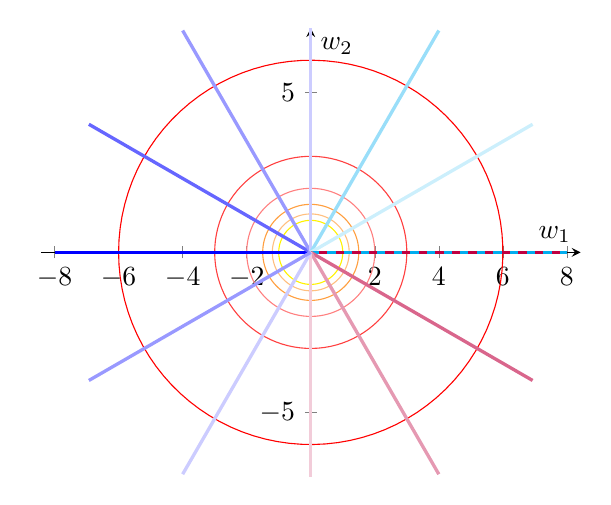
\begin{tikzpicture}
	\begin{axis}[
		axis lines=middle,
		axis equal,
		xmin=-7,
		xmax=7,
		ymin=-7,
		ymax=7,
		xlabel=$w_1$,
		ylabel=$w_2$,
	]	
		\addplot [domain=-180:180, samples=100, color=yellow] ({cos(x)/(cos(x)^2 + sin(x)^2}, {sin(x)/(cos(x)^2 + sin(x)^2});
		\addplot [domain=-180:180, samples=100, color=white!50!orange] ({(5/6*cos(x))/((5/6*cos(x))^2 + (5/6*sin(x))^2)}, {(5/6*sin(x))/((5/6*cos(x))^2 + (5/6*sin(x))^2)});
		\addplot [domain=-180:180, samples=100, color=white!25!orange] ({(4/6*cos(x))/((4/6*cos(x))^2 + (4/6*sin(x))^2)}, {(4/6*sin(x))/((4/6*cos(x))^2 + (4/6*sin(x))^2)});
		\addplot [domain=-180:180, samples=100, color=white!50!red] ({(3/6*cos(x))/((3/6*cos(x))^2 + (3/6*sin(x))^2)}, {(3/6*sin(x))/((3/6*cos(x))^2 + (3/6*sin(x))^2)});
		\addplot [domain=-180:180, samples=100, color=white!25!red] ({(2/6*cos(x))/((2/6*cos(x))^2 + (2/6*sin(x))^2)}, {(2/6*sin(x))/((2/6*cos(x))^2 + (2/6*sin(x))^2)});
		\addplot [domain=-180:180, samples=100, color=red] ({(1/6*cos(x))/((1/6*cos(x))^2 + (1/6*sin(x))^2)}, {(1/6*sin(x))/((1/6*cos(x))^2 + (1/6*sin(x))^2)});
		
		\addplot[-, blue, very thick] coordinates {(0, 0) (-8, 0)};
		\addplot[-, white!40!blue, very thick] coordinates {(0, 0) ({8*cos(150)}, {8*sin(150)})};
		\addplot[-, white!60!blue, very thick] coordinates {(0, 0) ({8*cos(120)}, {8*sin(120)})};
		\addplot[-, white!80!blue, very thick] coordinates {(0, 0) ({8*cos(90)}, {8*sin(90)})};
		\addplot[-, white!60!cyan, very thick] coordinates {(0, 0) ({8*cos(60)}, {8*sin(60)})};
		\addplot[-, white!80!cyan, very thick] coordinates {(0, 0) ({8*cos(30)}, {8*sin(30)})};
		
		\addplot[-, purple, very thick] coordinates {(0, 0) (8, 0)};
		\addplot[-, cyan, very thick, dashed] coordinates {(0, 0) (8, 0)};
		
		\addplot[-, white!40!purple, very thick] coordinates {(0, 0) ({8*cos(-30)}, {8*sin(-30)})};
		\addplot[-, white!60!purple, very thick] coordinates {(0, 0) ({8*cos(-60)}, {8*sin(-60)})};
		\addplot[-, white!80!purple, very thick] coordinates {(0, 0) ({8*cos(-90)}, {8*sin(-90)})};
		\addplot[-, white!80!blue, very thick] coordinates {(0, 0) ({8*cos(-120)}, {8*sin(-120)})};
		\addplot[-, white!60!blue, very thick] coordinates {(0, 0) ({8*cos(-150)}, {8*sin(-150)})};
	\end{axis}
\end{tikzpicture}
\end{tikzpicture}}
	\end{minipage}\\[3pt]

\subsection{Regeln bei der Kreisspiegelung}
	\fbox{
		\begin{tabular}{ll}
			\textbf{Winkeltreue:} & Die Kreisspiegelung ist \textbf{überall winkeltreu!}
		\end{tabular}
	}\\[3pt]
	\fbox{
		\begin{tabular}{ll}
			\textbf{Kreistreue:} & Die Kreisspiegelung ist kreistreu (Geraden sind Kreise mit $r = \infty$)
		\end{tabular}
	}\\[3pt]
	\begin{tabular}{|c|c|c|c|c|}
		\hline
		\textbf{Originalkurve:} & \textbf{Bildkurve:} & & \textbf{Originalkurve:} & \textbf{Bildkurve:}\\
		\hline
		\scalebox{0.5}{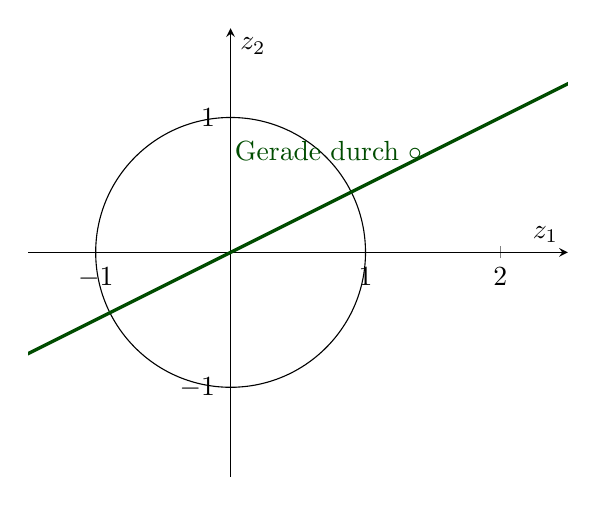
\begin{tikzpicture}
	\begin{axis}[
		axis lines=middle,
		axis equal,
		xmin=-1.5,
		xmax=2.5,
		ymin=-1,
		ymax=1,
		xlabel=$z_1$,
		ylabel=$z_2$,
	]	
		\draw (axis cs: 0, 0) circle [radius=1];
		\addplot[-, black!70!green, very thick] {0.5*x} node[above, left, black!70!green, pos=0.65] {Gerade durch $\circ$};
	\end{axis}
\end{tikzpicture}} & \scalebox{0.5}{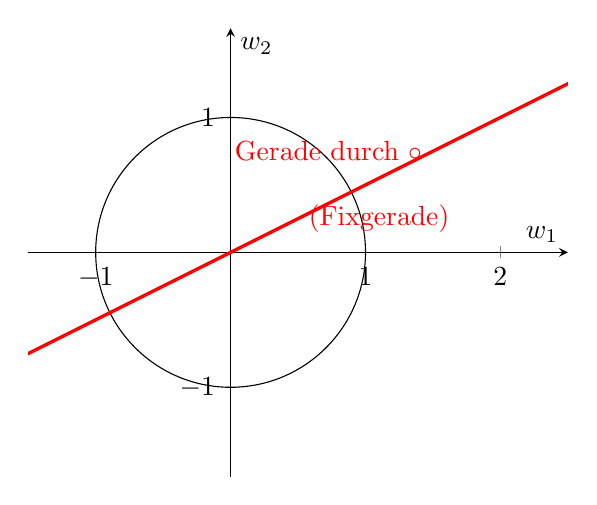
\begin{tikzpicture}
	\begin{axis}[
		axis lines=middle,
		axis equal,
		xmin=-1.5,
		xmax=2.5,
		ymin=-1,
		ymax=1,
		xlabel=$w_1$,
		ylabel=$w_2$,
		]	
		\draw (axis cs: 0, 0) circle [radius=1];
		\addplot[-, red, very thick] {0.5*x} node[above, left, red, pos=0.65] {Gerade durch $\circ$} node[below, right, red, pos=0.55] {(Fixgerade)};
	\end{axis}
\end{tikzpicture}} & & \scalebox{0.5}{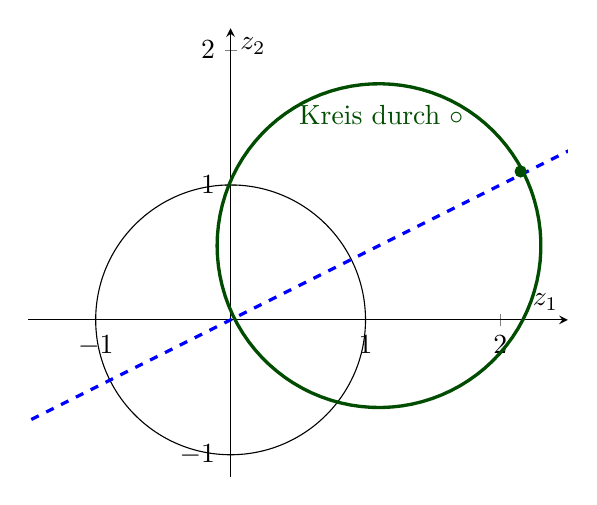
\begin{tikzpicture}
	\begin{axis}[
		axis lines=middle,
		axis equal,
		xmin=-1.5,
		xmax=2.5,
		ymin=-1,
		ymax=2,
		xlabel=$z_1$,
		ylabel=$z_2$,
	]	
		\draw (axis cs: 0, 0) circle [radius=1];
		\addplot[domain=-180:180, samples=100, color=black!70!green, very thick] ({1.2*cos(x) + 1.1}, {1.2*sin(x) + 0.55}) node[above, left, black!70!green, pos=0.65] {Kreis durch $\circ$};
		\addplot[-, blue, very thick, dashed] {0.5*x};
		\addplot[mark=*, black!70!green] coordinates {(2.15, 1.1)};
	\end{axis}
\end{tikzpicture}} & \scalebox{0.5}{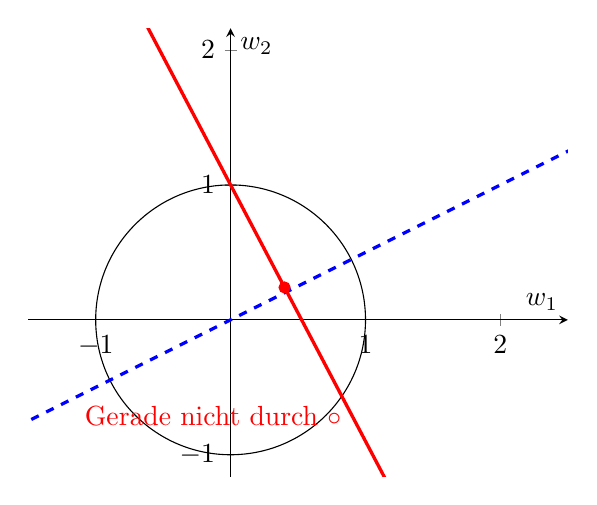
\begin{tikzpicture}
	\begin{axis}[
		axis lines=middle,
		axis equal,
		xmin=-1.5,
		xmax=2.5,
		ymin=-1,
		ymax=2,
		xlabel=$w_1$,
		ylabel=$w_2$,
		]	
		\draw (axis cs: 0, 0) circle [radius=1];
		\addplot[-, blue, very thick, dashed] {0.5*x};
		\addplot[-, red, very thick] {-1.9*x + 1} node[above, left, red, pos=0.59] {Gerade nicht durch $\circ$};
		\addplot[mark=*, red] coordinates {(0.4, 0.24)};
	\end{axis}
\end{tikzpicture}}\\
		\hline
		\scalebox{0.5}{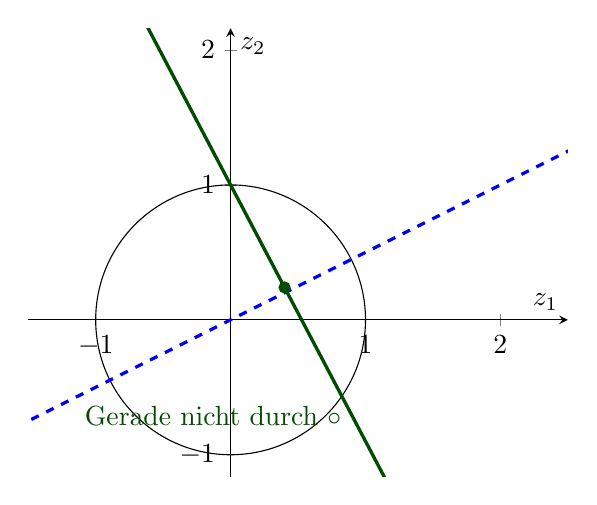
\begin{tikzpicture}
	\begin{axis}[
		axis lines=middle,
		axis equal,
		xmin=-1.5,
		xmax=2.5,
		ymin=-1,
		ymax=2,
		xlabel=$z_1$,
		ylabel=$z_2$,
		]	
		\draw (axis cs: 0, 0) circle [radius=1];
		\addplot[-, blue, very thick, dashed] {0.5*x};
		\addplot[-, black!70!green, very thick] {-1.9*x + 1} node[above, left, black!70!green, pos=0.59] {Gerade nicht durch $\circ$};
		\addplot[mark=*, black!70!green] coordinates {(0.4, 0.24)};
	\end{axis}
\end{tikzpicture}} & \scalebox{0.5}{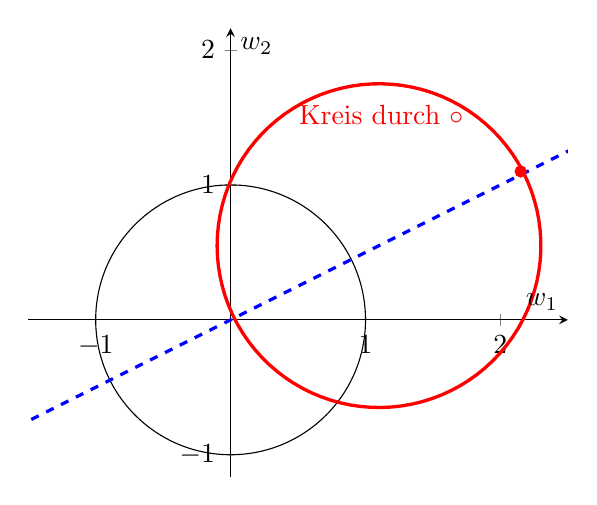
\begin{tikzpicture}
	\begin{axis}[
		axis lines=middle,
		axis equal,
		xmin=-1.5,
		xmax=2.5,
		ymin=-1,
		ymax=2,
		xlabel=$w_1$,
		ylabel=$w_2$,
	]	
		\draw (axis cs: 0, 0) circle [radius=1];
		\addplot[domain=-180:180, samples=100, color=red, very thick] ({1.2*cos(x) + 1.1}, {1.2*sin(x) + 0.55}) node[above, left, red, pos=0.65] {Kreis durch $\circ$};
		\addplot[-, blue, very thick, dashed] {0.5*x};
		\addplot[mark=*, red] coordinates {(2.15, 1.1)};
	\end{axis}
\end{tikzpicture}} & & \scalebox{0.5}{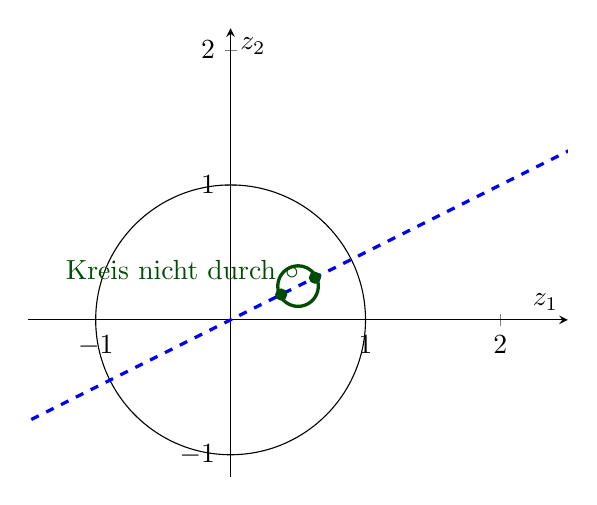
\begin{tikzpicture}
	\begin{axis}[
		axis lines=middle,
		axis equal,
		xmin=-1.5,
		xmax=2.5,
		ymin=-1,
		ymax=2,
		xlabel=$z_1$,
		ylabel=$z_2$,
	]	
		\draw (axis cs: 0, 0) circle [radius=1];
		\addplot[domain=-180:180, samples=100, color=black!70!green, very thick] ({0.15*cos(x) + 0.5}, {0.15*sin(x) + 0.25}) node[above, left, black!70!green, pos=0.65] {Kreis nicht durch $\circ$};
		\addplot[-, blue, very thick, dashed] {0.5*x};
		\addplot[mark=*, black!70!green] coordinates {(0.625, 0.3125)};
		\addplot[mark=*, black!70!green] coordinates {(0.375, 0.1875)};
	\end{axis}
\end{tikzpicture}} & \scalebox{0.5}{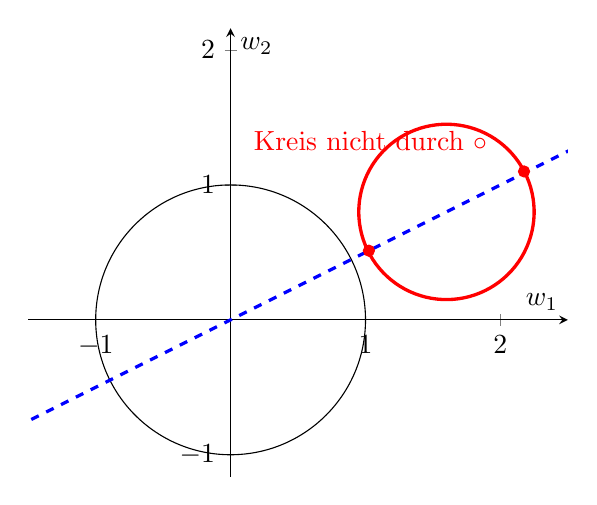
\begin{tikzpicture}
	\begin{axis}[
		axis lines=middle,
		axis equal,
		xmin=-1.5,
		xmax=2.5,
		ymin=-1,
		ymax=2,
		xlabel=$w_1$,
		ylabel=$w_2$,
	]	
		\draw (axis cs: 0, 0) circle [radius=1];
		\addplot[domain=-180:180, samples=100, color=red, very thick] ({0.65*cos(x) + 1.6}, {0.65*sin(x) + 0.8}) node[above, left, red, pos=0.65] {Kreis nicht durch $\circ$};
		\addplot[-, blue, very thick, dashed] {0.5*x};
		\addplot[mark=*, red] coordinates {(2.175, 1.1)};
		\addplot[mark=*, red] coordinates {(1.025, 0.5125)};
	\end{axis}
\end{tikzpicture}}\\
		\hline
	\end{tabular}\\[3pt]
	\begin{minipage}[t]{0.5\textwidth}
		\subsection{Konstruktion von Bildpunkten}
			\begin{tabular}{ll}
				$z$ \textbf{innerhalb des } & $z$ \textbf{ausserhalb des }\\[1pt] \textbf{Einheitskreises}: & \textbf{Einheitskreises}:\\[3pt]
				\scalebox{0.5}{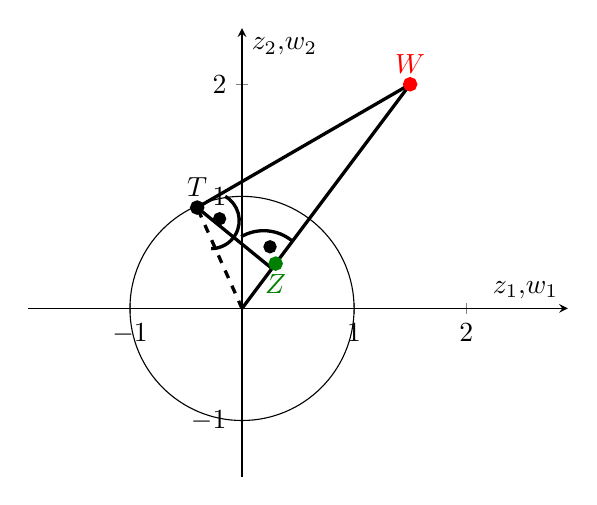
\begin{tikzpicture}
	\begin{axis}[
		axis lines=middle,
		axis equal,
		xmin=-0.5,
		xmax=1.5,
		ymin=-1.5,
		ymax=2.5,
		xlabel=$z_1\text{,} w_1$,
		ylabel=$z_2\text{,} w_2$,
		disabledatascaling
	]	
		\draw (axis cs: 0, 0) circle [radius=1];
		\addplot[-, very thick] coordinates {(0, 0) (1.5, 2)};
		\addplot[-, very thick] coordinates {(0.275, 0.35) (-0.4, 0.9)};
		\addplot[-, very thick] coordinates {(-0.4, 0.9) (1.5, 2)};
		\addplot[-, very thick, dashed] coordinates {(0, 0) (-0.4, 0.9)};
		\addplot[mark=*, very thick] coordinates {(-0.4, 0.9)} node[above] {$T$};
		\addplot[mark=*, very thick, black!50!green] coordinates {(0.3, 0.4)} node[below, black!50!green] {$Z$};
		\addplot[mark=*, very thick, red] coordinates {(1.5, 2)} node[above, red] {$W$};
		\draw [-, very thick] (axis cs:0.45, 0.6) arc [radius=0.4, start angle=50, end angle=120];
		\addplot[mark=*, thick] coordinates {(0.25, 0.55)};
		\draw [-, very thick] (axis cs:-0.15, 1) arc [radius=0.25, start angle=60, end angle=-90];
		\addplot[mark=*, thick] coordinates {(-0.2, 0.8)};
	\end{axis}
\end{tikzpicture}} & \scalebox{0.5}{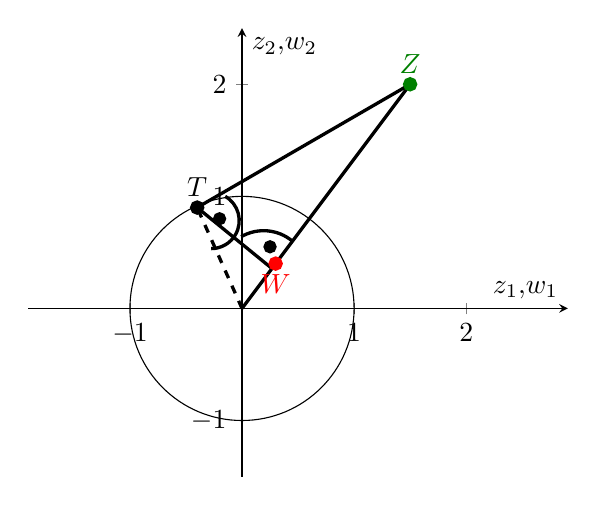
\begin{tikzpicture}
	\begin{axis}[
		axis lines=middle,
		axis equal,
		xmin=-0.5,
		xmax=1.5,
		ymin=-1.5,
		ymax=2.5,
		xlabel=$z_1\text{,} w_1$,
		ylabel=$z_2\text{,} w_2$,
		disabledatascaling
	]	
		\draw (axis cs: 0, 0) circle [radius=1];
		\addplot[-, very thick] coordinates {(0, 0) (1.5, 2)};
		\addplot[-, very thick] coordinates {(0.275, 0.35) (-0.4, 0.9)};
		\addplot[-, very thick] coordinates {(-0.4, 0.9) (1.5, 2)};
		\addplot[-, very thick, dashed] coordinates {(0, 0) (-0.4, 0.9)};
		\addplot[mark=*, very thick] coordinates {(-0.4, 0.9)} node[above] {$T$};
		\addplot[mark=*, very thick, black!50!green] coordinates {(1.5, 2)} node[above, black!50!green] {$Z$};
		\addplot[mark=*, very thick, red] coordinates {(0.3, 0.4)} node[below, red] {$W$};
		\draw [-, very thick] (axis cs:0.45, 0.6) arc [radius=0.4, start angle=50, end angle=120];
		\addplot[mark=*, thick] coordinates {(0.25, 0.55)};
		\draw [-, very thick] (axis cs:-0.15, 1) arc [radius=0.25, start angle=60, end angle=-90];
		\addplot[mark=*, thick] coordinates {(-0.2, 0.8)};
	\end{axis}
\end{tikzpicture}}
			\end{tabular}
	\end{minipage}
	\begin{minipage}[t]{0.5\textwidth}
		\subsection{Exponentialfunktion $\mathrm{e}^z$}
			\begin{minipage}[t]{0.3\textwidth}
				\fbox{$\mathrm{e} = \mathrm{e}^z_1 + \operatorname{cjs}\left( z_2 \right)$}
			\end{minipage}
			\begin{minipage}[t]{0.7\textwidth}
				\begin{tabular}{lcl}
					\textbf{Waagrechte} & $\rightarrow$ & \textbf{Strahlen}\\[3pt]
					\textbf{Senktrechte} & $\rightarrow$ & \textbf{Kreise um $\mathrm{O}$}\\[3pt]
				\end{tabular}
			\end{minipage}
			\scalebox{0.5}{\begin{tikzpicture}	
	\draw[->, very thick, red] (22:8cm) arc[radius=1, start angle=140, end angle=40] node[above, red] at (8.3, 3.3) {$w = \mathrm{e}^z$};
	
	\begin{tikzpicture}
	\begin{axis}[
		axis lines=middle,
		axis equal,
		xmin=-4,
		xmax=4,
		ymin=-4,
		ymax=4,
		xlabel=$z_1$,
		ylabel=$z_2$,
		axis background/.style={fill=gray!50}
	]
		\addplot[-, purple, line width=4pt] coordinates {({ln(1/3)}, -5) ({ln(1/3)}, 5)} node[below, left, pos=0.9] {$\ln\left( \dfrac{1}{3} \right)$};
		\addplot[-, blue, line width=4pt] coordinates {({ln(2/3)}, -5) ({ln(2/3)}, 5)} node[below, left, pos=0.2] {$\ln\left( \dfrac{2}{3} \right)$};
		\addplot[-, black!70!green, line width=4pt] coordinates {(0, -5) (0, 5)} node[below, right, pos=0.2] {$0$};
		\addplot[-, black!50!green, line width=4pt] coordinates {({ln(2)}, -5) ({ln(2)}, 5)} node[below, left, pos=0.9] {$\ln(2)$};
		\addplot[-, green, line width=4pt] coordinates {({ln(3)}, -5) ({ln(3)}, 5)} node[below, right, pos=0.2] {$\ln(3)$};
		
		\addplot[-, yellow, line width=4pt] coordinates {(-5, {5/6*pi}) (5, {5/6*pi})} node[below, left, pos=0.1] {$\dfrac{5}{6}\pi$};
		\addplot[-, orange, line width=4pt] coordinates {(0, {1/3*pi}) (5, {1/3*pi})} node[below, left, pos=0.7] {$\dfrac{1}{3}\pi$};
		\addplot[-, red, line width=4pt] coordinates {(-5, 0) (0, 0)};
		\addplot[-, black!50!red, line width=4pt] coordinates {(-5, {-1/3*pi}) (0, {-1/3*pi})} node[below, left, pos=0.7] {$-\dfrac{1}{3}\pi$};
		\addplot[-, purple, line width=4pt] coordinates {(-5, {-5/6*pi}) (5, {-5/6*pi})} node[below, right, pos=0.7] {$\dfrac{5}{6}\pi$};
	\end{axis}
\end{tikzpicture}\hspace{2.7cm}%
	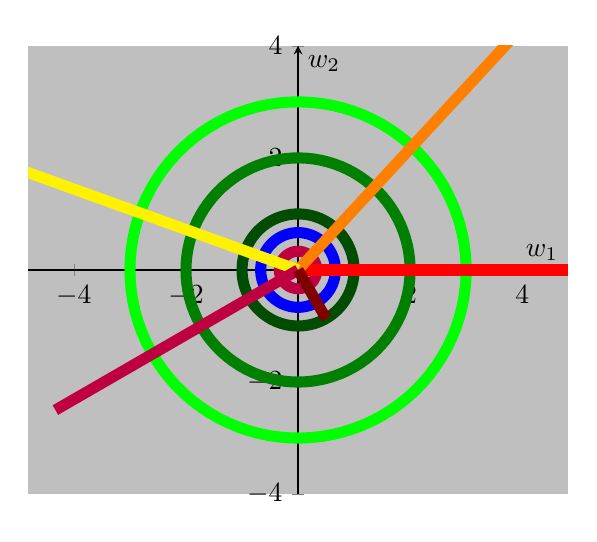
\begin{tikzpicture}
	\begin{axis}[
		axis lines=middle,
		axis equal,
		xmin=-4,
		xmax=4,
		ymin=-4,
		ymax=4,
		xlabel=$w_1$,
		ylabel=$w_2$,
		axis background/.style={fill=gray!50}
	]	
		\addplot [domain=-180:180, samples=100, color=green, line width=4pt] ({3*cos(x)}, {3*sin(x)});
		\addplot [domain=-180:180, samples=100, color=black!50!green, line width=4pt] ({2*cos(x)}, {2*sin(x)});
		\addplot [domain=-180:180, samples=100, color=black!70!green, line width=4pt] ({cos(x)}, {sin(x)});
		\addplot [domain=-180:180, samples=100, color=blue, line width=4pt] ({2/3*cos(x)}, {2/3*sin(x)});
		\addplot [domain=-180:180, samples=100, color=purple, line width=4pt] ({1/3*cos(x)}, {1/3*sin(x)});
		
		\addplot[-, red, line width=4pt] coordinates {(0, 0) (5, 0)};
		\addplot[-, orange, line width=4pt] coordinates {(0, 0) ({8*cos(60)}, {5*sin(60)})};
		\addplot[-, yellow, line width=4pt] coordinates {(0, 0) ({8*cos(150)}, {5*sin(150)})};
		\addplot[-, purple, line width=4pt] coordinates {(0, 0) ({5*cos(-150)}, {5*sin(-150)})};
		\addplot[-, black!50!red, line width=4pt] coordinates {(0, 0) ({cos(-60)}, {sin(-60)})};
	\end{axis}
\end{tikzpicture}
\end{tikzpicture}}
	\end{minipage}